% -- Slide ---------------------------------------------------------------------
\begin{frame}
\frametitle{\bf Outline}

  
\includegraphics[height=0.5in]{images/tachyon-icon.png}
  \begin{minipage}[b]{3.5in}
    \begin{center}
      {\em Tachyon:~~~~~~~~~~~~~~~~~~~~~~~~~~~~~~~~~~~~~~~~~~~~~~~~~~~~~~~~~\\ a hypothetical particle that travels faster than light.} \\
      -- Oxford Dictionary
    \end{center}
  \end{minipage}

  \bigskip

  \begin{itemize}

  \item {\bf System overview} -- {\em Marc Feeley}
    \smallskip

  \item {\bf IR and optimization} -- {\em Maxime Chevalier-Boisvert}
    \smallskip

  \item {\bf Back-end, profiling and benchmarks} -- {\em Bruno Dufour}
    \smallskip

  \end{itemize}

  \bigskip
  \bigskip

  Unfortunately {\em Erick Lavoie} could not be here (responsible
  for back-end and register allocator)

\end{frame}
% ------------------------------------------------------------------------------

% -- Slide ---------------------------------------------------------------------
\begin{frame}
\frametitle{\bf Goals}

  \begin{itemize}

  \item Tachyon JS project started March 2010
    \smallskip

  \item JS is a key language with a bright future
    \smallskip

  \item 2010 JS VMs performance... {\bf We can do better!}
    \smallskip

    \bigskip

  \item Goal \#1: compiler for {\bf research on dynamic languages}
    \begin{itemize}
    \item optimistic optimization
    \item object representation / garbage collection
    \item profiling real-world applications
    \item language extensions: exact arithmetic, continuations, tail calls, exceptions, concurrency, distributed computing, Harmony,~...
    \item {\bf must stay flexible!} e.g.~calling protocol, object layout, ...
    \end{itemize}
    \smallskip

  \item Goal \#2: {\bf production-quality} high-performance open-source
    JS compiler for client-side and server-side scripting

  \end{itemize}

\end{frame}
% ------------------------------------------------------------------------------

% -- Slide ---------------------------------------------------------------------
\begin{frame}
\frametitle{\bf Self-Hosting in a Dynamic Language}

  \begin{itemize}

  \item JIT compilers are efficient because they
    \begin{itemize}
      \item[1.] compile the program parts where speed matters
      \item[2.] {\bf adapt/specialize the program} to the run time conditions
    \end{itemize}
    \smallskip

  \item {\bf Particularly useful to speed up dynamic languages}
    \smallskip

  \item {\bf Dynamic compilation may outperform static compilation}
    \smallskip

  \item ... but only if {\bf compilation time is kept small}
    \begin{itemize}
    \item avoid expensive optimizations
    \item use hand-tuned algorithms
    \item break abstraction barriers
    \end{itemize}
    \smallskip

  \item {\bf Not obvious when host is a dynamic language!}

  \end{itemize}
\end{frame}
% ------------------------------------------------------------------------------

% -- Slide ---------------------------------------------------------------------
\begin{frame}
\frametitle{\bf Self-Hosting JIT Thesis}

  \begin{itemize}

  \item Our idea: {\bf dynamically recompile the JIT compiler}
    \bigskip
    \bigskip

  \item {\bf Adapts the JIT compiler to the program being compiled}
    \smallskip

  \item The cost of JIT compiler adaptation is amortized over
    {\bf repeated recompilations of the same program}
    \smallskip

  \item Host language must also be JIT compiled... {\bf Recursion!}
    \bigskip

  \item Other self-hosting benefits:
    \begin{itemize}
      \item single runtime system (one heap, GC, I/O, ...)
      \item easy introspection and dynamic language extension
      \item we are more productive in JS than C/C++!
    \end{itemize}
    \smallskip

  \end{itemize}
\end{frame}
% ------------------------------------------------------------------------------

% -- Slide ---------------------------------------------------------------------
\begin{frame}
\frametitle{\bf Current State}

  \begin{itemize}

  \item Compiler is written in a subset of JS (roughly 40 KLOC):
    \begin{itemize}
    \item parsing
    \item analysis/optimization of IR
    \item linear-scan reg.~alloc.
    \item assembler and linker for {\bf x86} and {\bf x86\_64}
    \item stdlib in JS
    \end{itemize}
    \smallskip

  \item Implements ES5 spec except:
    \begin{itemize}
    \item floating point (only fixnums are supported)
    \item regular expressions
    \item getters and setters, property attributes
    \item {\tt eval} and most meta-object protocol features
    \item no GC yet!
    \end{itemize}
    \smallskip

  \item Goodies: interactive shell, profiler, benchmarking framework
    \smallskip

  \item March 2011: Tachyon self-bootstrap using V8
    \smallskip

  \end{itemize}
\end{frame}
% ------------------------------------------------------------------------------

%
% Slide about compilation phases, with graphic
%
\begin{frame}
\frametitle{\bf Tachyon Compiler Pipeline}
\begin{center}
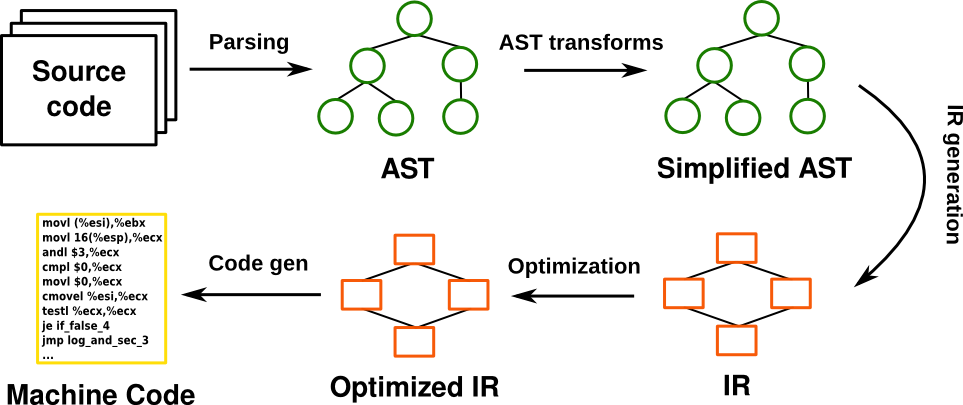
\includegraphics[width=4.5in]{images/phases}
\end{center}
\end{frame}

% -- Slide ---------------------------------------------------------------------
\begin{frame}
\frametitle{\bf Parser}

  \begin{itemize}

  \item Based on WebKit's yacc grammar
    \begin{itemize}
    \item {\tt Grammar.y} converted to LALR-SCM parser generator spec
    \item LALR-SCM tables pretty-printed as JS arrays (6 KLOC)
    \item hand written scanner (1 KLOC) and LALR driver (.3 KLOC)
    \end{itemize}
    \smallskip

  \item Parses 100 KLOC per second
    \smallskip

  \item Source location attached to all AST nodes

  \end{itemize}

  \begin{center}
    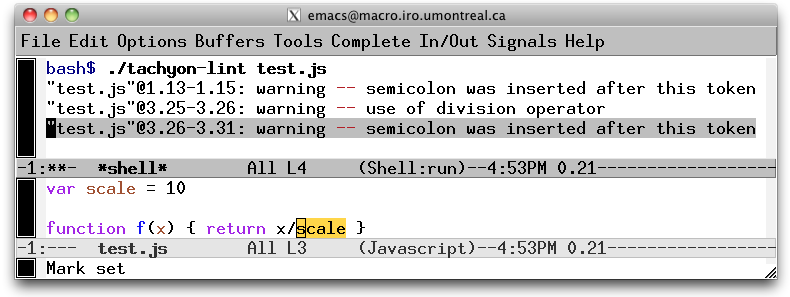
\includegraphics[height=1.5in]{images/tachyon-lint.png}
  \end{center}

\end{frame}
% ------------------------------------------------------------------------------

% -- Slide ---------------------------------------------------------------------
\begin{frame}[fragile]
\frametitle{\bf Parser Derivatives for Debugging}

  \begin{itemize}

  \item {\bf JS pretty-printer} -- dump or pretty print AST
    \smallskip

  \item {\bf js2scm} -- compile JS to Scheme
    \smallskip

  \item {\bf js2js} -- instrument JS code with function entry/exit tracing
    \smallskip

\begin{lstlisting}[language=]
bash$ ./js2js -debug tachyon.js > tachyon-debug.js
bash$ d8 tachyon-debug.js
|  (( "utility/iterators.js"@13.1-17.2: Iterator
|  |  (( "utility/debug.js"@73.1-77.2: assertNew
|  |  |  (( "utility/debug.js"@62.1-68.2: isGlobal
|  |  |  |  (( "utility/debug.js"@65.19-65.47: isGlobal
|  |  |  |  )) "utility/debug.js"@65.33-65.45: isGlobal
|  |  |  )) "utility/debug.js"@67.5-67.27: isGlobal
|  |  )) "utility/debug.js"@73.1-77.2: assertNew
|  )) "utility/iterators.js"@16.5-16.17: Iterator
|  (( "utility/iterators.js"@13.1-17.2: Iterator
|  |  (( "utility/debug.js"@73.1-77.2: assertNew
...
\end{lstlisting}

  \end{itemize}

\end{frame}
% ------------------------------------------------------------------------------

% -- Slide ---------------------------------------------------------------------
\begin{frame}[fragile]
\frametitle{\bf AST Transformations}

  \begin{itemize}
  \item Simplification of AST
  \item Resolve scopes and compute free variables
  \item Detect uses of \code{eval} and \code{arguments}
  \end{itemize}
  \bigskip

\begin{lstlisting}[keepspaces=true]
// rewrite property access
obj.prop  ==>  obj["prop"]

// variable declaration hoisting to function top
function f(...) {        for (var x = E; ...) ... }  ==>
function f(...) { var x; for (    x = E; ...) ... }

// alias parameters to arguments object
function f(x,y) {            ... arguments ...; x = y; }  ==>
function f()    { var a = arguments; ... a ...; a[0] = a[1]; }
\end{lstlisting}

\end{frame}
% ------------------------------------------------------------------------------
